\documentclass[a4paper,12pt,oneside]{article}
\usepackage{amsmath}
%\usepackage{mathtools}
\usepackage{caption}
\usepackage{mathptmx}
\usepackage{etoolbox}
\usepackage{graphicx}
\usepackage[margin=1.0in]{geometry}
\usepackage{float}
\usepackage{setspace}
\usepackage{chngcntr}
\usepackage{fancyhdr}
\pagestyle{fancy}
\fancyhf{}
\rfoot{\thepage}
%\renewcommand{\headrulewidth}{0.0pt}
%\renewcommand{\footrulewidth}{0.0pt}

\begin{document}
\thispagestyle{empty}
%\pagenumbering{gobble}
\begin{center}
\vspace*{4mm}
\large{\textbf{Gradual Relaxation Suggestions using Facial Expression Recognition}
\setlength{\baselineskip}{1.5\baselineskip}}
\\

\vspace{5mm}
\textbf{PROJECT REPORT}
\\
\vspace{3mm}
Submitted in the partial fulfilment of the award of the degree
of
\vspace{3mm}
\\
\textbf{Bachelor of Technology}
\\
\vspace{3mm}
in
\\
\vspace{3mm}
\textbf{Computer Science \& Engineering}
\\
\vspace{3mm}
of
\\
\vspace{3mm}
\textbf{APJ Abdul Kalam Technological University}
\\
\vspace{3mm}
by
\\
\vspace{3mm}
\textbf{Abhishek S}
\\
\textbf{Gokul V Namboothiri}
\\
\textbf{Nobin Jacob}
\\
\textbf{Sebin George Varghese}
\\
\vspace{5mm}

\begin{figure}[H]
	\centering
	
\includegraphics{ceclogo.png}
\end{figure}

\vspace{21mm}
\textbf{May, 2018}
\vspace{8mm}
\\
\vspace{2mm}
Department of Computer Engineering
\\
\vspace{2mm}
College of Engineering, Chengannur, Kerala -689121
\\
\vspace{2mm}
Phone: (0479) 2454125, 2451424; Fax: (0479) 2451424
\\
\end{center}

\newpage
\thispagestyle{empty}
\begin{center}
\setlength{\baselineskip}{1.5\baselineskip}
{\large\textbf{COLLEGE OF ENGINEERING, CHENGANNUR}}
\\
{\large\textbf{KERALA}}
\vspace{4mm}
\begin{figure}[H]
\centering

\includegraphics{ceclogo.png}
\end{figure}
\setlength{\baselineskip}{1.5\baselineskip}
\textbf{Department of Computer Engineering}
\\
\textbf{CERTIFICATE}
\\
This is to certify that the project entitled
\\
\textbf{Gradual Relaxation Suggestions using Facial Expression Recognition}
\\
Submitted by
\\
\textbf{Abhishek S}
\\
\textbf{Gokul V Namboothiri}
\\
\textbf{Nobin Jacob}
\\
\textbf{Sebin George Varghese}
\\
is a bonafide record of the work done by them.
\end{center}
\vspace{2ex}
\vspace{10ex}
%\textbf{Mrs.Shiny}
\hspace{55ex}
%\textbf{Dr. Smitha Dharan}
\\
\vspace{2ex}
\hspace{5ex}
\textbf{
Co-ordinator}
\hspace{40ex}
\textbf{
Head of The Department}
\\
\\
\\
\begin{center}
\textbf{
Guide}
\end{center}

\newpage
\pagenumbering{roman}
\renewcommand{\headrulewidth}{0.0pt}
\renewcommand{\footrulewidth}{0.0pt}
\begin{center}
\large{\textbf{ACKNOWLEDGEMENT}}
\end{center}
\vspace{4ex}
\setlength{\baselineskip}{1.5\baselineskip}

\paragraph{}
We are greatly indebted to God Almighty for being the guiding light throughout with his
abundant grace and blessings that strengthened us to do this endeavour with confidence.
\paragraph{}
We express our heartfelt gratitude towards \textbf{Dr. Jacob Thomas V.}, Principal, College
of Engineering Chengannur for extending all the facilities required for doing our project.
We would also like to thank \textbf{Dr. Smitha Dharan}, Head, Department of Computer
Engineering, for providing constant support and encouragement.
\paragraph{}
Now we extend our sincere thanks to our project co-ordinators \textbf{Mrs. Shiny B}, Assistant
Professor in Computer Engineering , \textbf{Ms. Archana Vijayan} , Assistant
Professor in Computer Engineering and  \textbf{Mrs. C Jyothirmayi Devi}, Assistant Professor in Computer Engineering for guiding us in our work and providing timely advices and valuable suggestions.
\paragraph{}
Last but not the least, we extend our heartfelt gratitude to our parents and friends for
their support and assistance.	

\pagenumbering{gobble}
\newpage

\begin{center}
\large{\textbf{ABSTRACT}}
\end{center}
\vspace{6ex}
\paragraph{}
A Facial expression is the visible manifestation of the affective state, cognitive activity,
intention, personality and psychopathology of a person and plays a communicative role in
interpersonal relations. Automatic recognition of facial expressions can be an important
component of  natural  human-machine  interfaces;  it  may  also  be  used  in behavioral  science
and  in  clinical  practice. An automatic Facial Expression Recognition system needs to perform
detection and location of faces in a cluttered scene, facial feature extraction, and facial
expression classification.
\paragraph{}
Facial expression recognition system is implemented using Convolution Neural Network
(CNN). CNN model of the project is based on LeNet Architecture. Kaggle facial expression
dataset with seven facial expression labels as happy, sad, surprise, fear, anger, disgust, and
neutral is used in this project. The system achieved 56.77 \% accuracy and 0.57 precision on
testing dataset.
\setlength{\baselineskip}{1.0\baselineskip}

\newpage
\begin{center}
\tableofcontents
\end{center}

\newpage
\thispagestyle{plain}
\begin{center}
\vspace{5mm}
\listoffigures
\vspace{5mm}
\end{center}


\newpage
\rfoot{\thepage}

\lhead{\textit{Gradual Relaxation Suggestions using Facial Expression Recognition}}

\lfoot{\textit{College of Engineering, Chengannur}}

\rfoot{\thepage}

\renewcommand{\headrulewidth}{0.0pt}
\renewcommand{\footrulewidth}{0.0pt}

\section{Overview}
\subsection{Background}
\pagenumbering{arabic}
\paragraph{}
A Facial expression is the visible manifestation of the affective state, cognitive activity, intention, personality and psychopathology of a person and plays a communicative role in interpersonal relations. Human facial expressions can be easily classified into 7 basic emotions: happy, sad, surprise, fear, anger, disgust, and neutral. Our facial emotions are expressed through activation of specific sets of facial muscles. These sometimes subtle, yet complex, signals in an expression often contain an abundant amount of information about our state of mind.  
\paragraph{}
Automatic recognition of facial expressions can be an important component of  natural  humanmachine  interfaces;  it  may  also  be  used  in behavioral  science  and  in  clinical  practice. It have been studied for a long period of time and obtaining the progress recent decades. Though much progress has been made, recognizing facial expression with a high accuracy remains to be difficult due to the complexity and varieties of facial expressions.
\paragraph{}
On a day to day basics humans commonly recognize emotions by characteristic features, displayed as a part of a facial expression. For instance happiness is undeniably associated with a smile or an upward movement of the corners of the lips. Similarly other emotions are characterized by other deformations typical to a particular expression. Research into automatic recognition of facial expressions addresses the problems surrounding the representation and categorization of static or dynamic characteristics of these deformations of face pigmentation .    
\paragraph{}
In machine learning, a convolutional neural network (CNN, or ConvNet) is a type of feedforward artificial neural network in which the connectivity pattern between its neurons is inspired by the organization of the animal visual cortex. Individual cortical neurons respond to stimuli in a restricted region of space known as the receptive field. The receptive fields of different neurons partially overlap such that they tile the visual field. The response of an individual neuron to stimuli within its receptive field can be approximated mathematically by a convolution operation. Convolutional networks were inspired by biological processes and are variations of multilayer perceptron designed to use minimal amounts of preprocessing.
\paragraph{}
They have wide applications in image and video recognition, recommender systems and natural language processing. The convolutional neural network is also known as shift invariant or space invariant artificial neural network (SIANN), which is named based on its shared weights architecture and translation invariance characteristics. 
\paragraph{}
LeNet is one of the very first convolutional neural networks which helped propel the field of Deep Learning. This pioneering work by Yann LeCun was named LeNet5 was used mainly for character recognition tasks such as reading zip codes, digits, etc. The basic architecture of LeNet can be shown as below:

\begin{figure}[H]
\centering
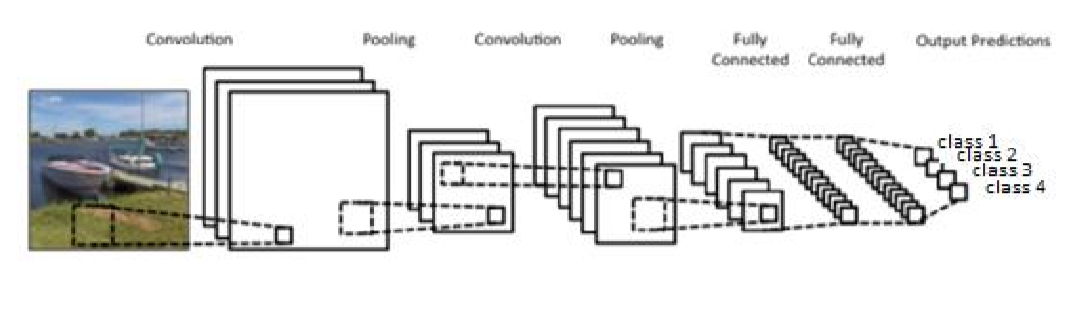
\includegraphics[height=7cm,width=17cm]{1.png}
\counterwithin{figure}{section}
\caption{A Brief model of CNN}
%\counterwithout{figure}{chapter}
\end{figure}

\paragraph{}
There are four main operations in the Convolution Neural Network shown in Figure 2.2 above:  

\subsubsection{Convolution:}
\paragraph{}
The primary purpose of Convolution in case of a CNN is to extract features from the input
image. Convolution preserves the spatial relationship between pixels by learning image
features using small squares of input data. The convolution layer’s parameters consist of a set
of learnable filters. Every filter is small spatially (along width and height), but extends through
the full depth of the input volume. For example, a typical filter on a first layer of a CNN might
have size 3x5x5 (i.e. images have depth 3 i.e. the color channels, 5 pixels width and height).
During the forward pass, each filter is convolved across the width and height of the input
volume and compute dot products between the entries of the filter and the input at any position.
As the filter convolve over the width and height of the input volume it produces a 2-dimensional
activation map that gives the responses of that filter at every spatial position. Intuitively, the
network will learn filters that activate when they see some type of visual feature such as an edge of some orientation or a blotch of some color on the first layer, or eventually entire
honeycomb or wheel-like patterns on higher layers of the network. Now, there will be an entire
set of filters in each convolution layer (e.g. 20 filters), and each of them will produce a separate
2-dimensional activation map.
\paragraph{}
The 2-dimensional convolution between image A and Filter B can be given as:

\begin{figure}[H]
\centering
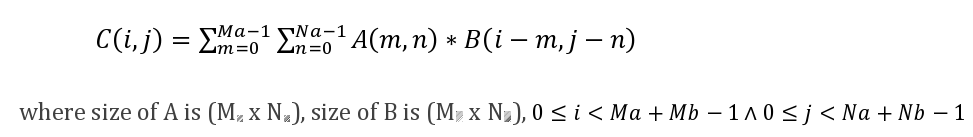
\includegraphics[height=3cm,width=17cm]{1a.png}
\counterwithin{figure}{section}
\caption{2D convolution}
%\counterwithout{figure}{chapter}
\end{figure}

\paragraph{}
A filter convolves with the input image to produce a feature map. The convolution of another
filter over the same image gives a different feature map. Convolution operation captures the
local dependencies in the original image. A CNN learns the values of these filters on its own
during   the   training   process (althoug parameters such as number of filters, filter
size, architecture of the network etc. still needed to specify before the training process).The
more number of filters, the more image features get extracted and the better network becomes
at recognizing patterns in unseen images.
\paragraph{}
The size of the Feature Map (Convolved Feature) is controlled by three parameters:
\begin{itemize}
	\item Depth: Depth corresponds  to  the  number  of  filters  we use  for  the  convolution.
operation.
	\item Stride: Stride is the size of the filter, if the size of the filter is 5x5 then stride is 5.
	\item Zero-padding: Sometimes, it is convenient to pad the input matrix with zeros around
the border, so that filter can be applied to bordering elements of input image matrix.
Using zero padding size of the feature map can be controlled.
\end{itemize}

\subsubsection{Rectified Linear Unit}
\paragraph{}
An additional operation called ReLU has been used after every Convolution operation. A
Rectified Linear Unit (ReLU) is a cell of a neural network which uses the following activation
function to calculate its output given x:
\paragraph{}
R(x)=Max(0,x)
\paragraph{}
Using these cells is more efficient than sigmoid and still forwards more information compared
to binary units. When initializing the weights uniformly, half of the weights are negative. This helps creating a sparse feature representation. Another positive aspect is the relatively cheap
computation. No exponential function has to be calculated. This function also prevents the
vanishing gradient error, since the gradients are linear functions or zero but in no case non-
linear functions.
\vspace{0.5cm}

\subsubsection{Pooling(sub-sampling)}
\paragraph{}
Spatial Pooling (also called subsampling or downsampling) reduces the dimensionality of each
feature map but retains the most important information. Spatial Pooling can be of different
types: Max, Average, Sum etc. In case of Max Pooling, a spatial neighborhood (for example, a
2×2 window) is defined and the largest element is taken from the rectified feature map within
that window. In case of average pooling the average or sum of all elements in that window is
taken. In practice, Max Pooling has been shown to work better.
\paragraph{}
Max Pooling reduces the input by applying the maximum function over the input xi. Let m be
the size of the filter, then the output calculates as follows:
\vspace{0.5cm}

\begin{figure}[H]
\centering
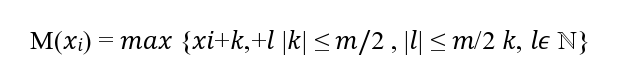
\includegraphics[height=2cm,width=09cm]{1b.png}
\counterwithin{figure}{section}
\caption{Max pooling Eq}
%\counterwithout{figure}{chapter}
\end{figure}

\begin{figure}[H]
\centering
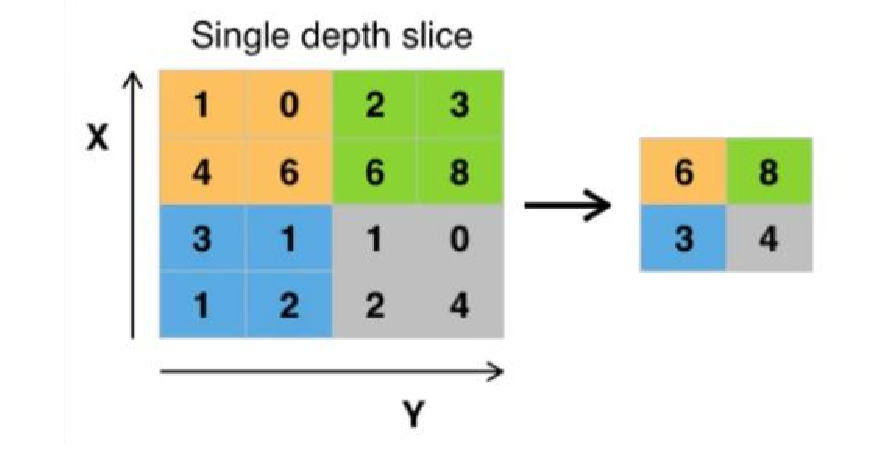
\includegraphics[height=07cm,width=14cm]{2.png}
\counterwithin{figure}{section}
\caption{Max pooling representaion}
%\counterwithout{figure}{chapter}
\end{figure}

\paragraph{}
The function of Pooling is to progressively reduce the spatial size of the input representation.
In particular, pooling;
\begin{itemize}
	\item Makes the input representations (feature dimension) smaller and more manageable.
	\item Reduces the number of parameters and computations in the network, therefore,
controlling over-fitting
	\item Makes the network invariant to small transformations, distortions and translations in
the input image (a small distortion in input will not change the output of Pooling.
	\item Helps us arrive at an almost scale invariant representation. This is very powerful since
objects can be detected in an image no matter where they are located.
\end{itemize}

\subsubsection{Classification(Multilayer Perceptron)}
\paragraph{}
The Fully Connected layer is a traditional Multi-Layer Perceptron that uses a softmax
activation function in the output layer. The term “Fully Connected” implies that every neuron
in the previous layer is connected to every neuron on the next layer. The output from the
convolutional and pooling layers represent high-level features of the input image. The purpose
of the Fully Connected layer is to use these features for classifying the input image into various
classes based on the training dataset.
\paragraph{}
Softmax is used for activation function. It treats the outputs as scores for each class. In the
Softmax, the function mapping stayed unchanged and these scores are interpreted as the un-
normalized log probabilities for each class. Softmax is calculated as: f(zj); where j is index for image and K is number of total facial expression class.
\paragraph{}
Apart from classification, adding a fully-connected layer is also a (usually) cheap way of
learning non-linear combinations of these features. Most of the features from convolutional
and pooling layers may be good for the classification task, but combinations of those features
might be even better.
\paragraph{}
The sum of output probabilities from the Fully Connected Layer is 1. This is ensured by using
the  as the activation function in the output layer of the Fully Connected Layer. The Softmax
function takes a vector of arbitrary real-valued scores and squashes it to a vector of values
between zero and one that sum to one.

\subsection{Problem Definition}
\paragraph{}
Human emotions and intentions are expressed through facial expressions and deriving an
efficient and effective feature is the fundamental component of facial expression system. Facial
expressions  convey  non-verbal  cues,  which play  an  important  role  in  interpersonal
relations.  Automatic recognition of facial expressions can be an important component of
natural  human-machine  interfaces;  it  may  also  be  used  in behavioral  science  and  in
clinical  practice. An automatic Facial Expression Recognition system needs to solve the
following problems: detection and location of faces in a cluttered scene, facial feature
extraction, and facial expression classification.
\subsection{Objective}
The objective of the project is:

\begin{itemize}
	\item To implement Convolutional Neural Networks for classification of facial expressions.
\end{itemize}

\subsection{Scope of the Project}
\paragraph{}
In this project facial expression recognition system is implemented using convolution neural
network to analyze the human state information to suggest  relaxation techniques such as a movie that matches or overcomes his/her current state of mind. Facial images are classified into seven facial expression categories namely Anger,
Disgust, Fear, Happy, Sad, Surprise and 'Neutral. Kaggle dataset is used to train and test the
classifier. These seven categories of experssions are used to identify which genre of movie is perfect for a human


\newpage
\section{Literature Review}
\paragraph{}
Two different approaches are used for facial expression recognition, both of which include two
different methodologies, exist [6].  Dividing the face into separate action units or keeping it as
a whole for further processing appears to be the first and the primary distinction between the
main approaches.  In both of these approaches, two different methodologies, namely the
‘Geometric based’ and the ‘Appearance-based’ parameterizations, can be used.
\paragraph{}
Making use of the whole frontal face image and processing it in order to end up with the
classifications of 6 universal facial expression prototypes: disgust, fear, joy, surprise, sad ness
and anger; outlines the first approach. Here, it is assumed that each of the above mentioned
emotions have characteristic expressions on face and that’s why recognition of them is
necessary and sufficient. Instead of using the face images as a whole, dividing them into some
sub-sections for further processing forms up the main idea of the second approach for facial
expression analysis. As expression is more related with subtle changes of some discrete
features such as eyes, eyebrows and lip corners; these fine-grained changes are used for
analyzing automated recognition.
\paragraph{}
There are two main methods that are used in both of the above explained approaches. Geometric
Based Parameterization is an old way which consists of tracking and processing the motions
of some spots on image sequences, firstly presented by Suwa et al to recognize facial
expressions [7]. Cohn and Kanade later on tried geometrical modeling and tracking of facial
features by claiming that each AU is presented with a specific set of facial muscles [8]. The
disadvantages of this method are the contours of these features and components have to be
adjusted manually in this frame, the problems of robustness and difficulties come out in cases
of pose and illumination changes while the tracking is applied on images, as actions \&
expressions tend to change both in morphological and in dynamical senses, it becomes hard to
estimate general parameters for movement and displacement. Therefore, ending up with robust
decisions for facial actions under these varying conditions becomes to be difficult.
\paragraph{}
Rather than tracking spatial points and using positioning and movement parameters that vary
within time, color (pixel) information of related regions of face are processed in Appearance
Based Parameterizations; in order to obtain the parameters that are going to form the feature vectors. Different features such as Gabor, Haar wavelet coefficients, together with feature
extraction and selection methods such as PCA, LDA, and Adaboost are used within this
framework.
\paragraph{}
For classification problem, algorithms like Machine learning, Neural Network, Support Vector
Machine, Deep learning, Naive Bayes are used.
\paragraph{}
Raghuvanshi A. et al have built a Facial expression recognition system upon recent research to
classify images of human faces into discrete emotion categories using convolutional neural
networks [9]. Alizadeh, Shima, and Azar Fazel have developed Facial Expression Recognition
system using Convolutional Neural Networks based on Torch model.

\subsection{Previous Technology}

\paragraph{}
This system is recently developed by the radar community to detect the moving object
behind the wall which give moving blobs as a result for the moving object behind the wall. This
system separates reflection from wall or other static object and the reflection from moving object
behind the wall based on their arrival time, so it must required to identify delays of even subnanoseconds.

\paragraph{}
The system shown above in Fig requires 2GHz of bandwidth, a very large power
source, and around 8-foot long antenna array and most important parameter is that the large
power in such a wide spectrum is infeasible for entities other than the military application.
\subsection{WISEE}
\paragraph{}
WISEE is a gesture recognition system that utilizes wireless signals to recognition of
human gesture. This system can recognize the human gesture without requiring any sensing
device on the human body. The required prototype for WISEE system is developed using USRPN210.

\begin{figure}[H]
\centering
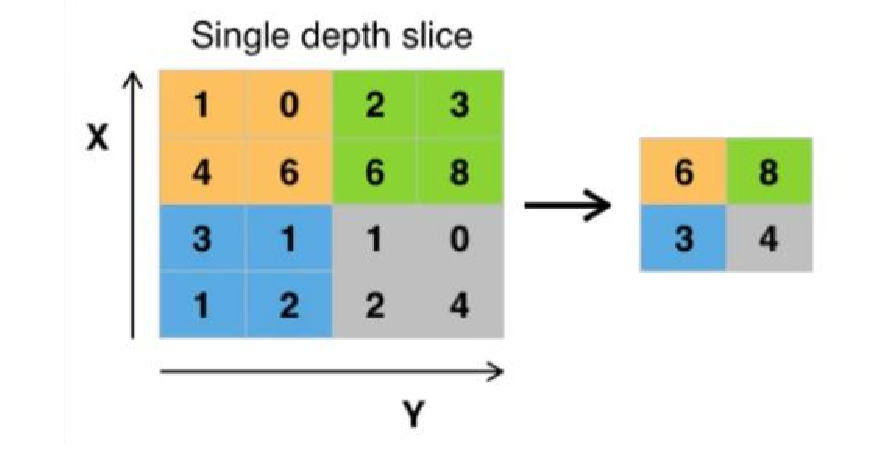
\includegraphics[height=5cm,width=12cm]{2.png}
\counterwithin{figure}{section}
\caption{WISEE}
%\counterwithout{figure}{chapter}
\end{figure}

\paragraph{}
 WISEE system use the property of Doppler shift, Doppler shift is the frequency change
of transmitted wave as its source moves relative to the observer. There will be multipath
reflection from the human body, and then human gestures results in pattern of Doppler shift at
the system receiver. So, the movement of user away from the receiver results in negative Doppler
shift, and movement of user towards the receiver results in positive Doppler shift. The challenge
for this system was that result of the human gesture gives very small change in Doppler shifts
that can be very hard to detect from WI-FI transmission. Typically movement around 0.5 m/sec
results in 17 Hz Doppler shift for the 5 GHz WI-FI transmission. For the gesture recognition it is
required to detect the Doppler shifts of few Hertz from 20 MHz WI-FI signals. This solution of
this problem is achieved by transforming the signal which are received from moving object, in to
narrowband pulse with a bandwidth of few Hertz, then system tracks the frequency of this
narrowband pulses to detect the small Doppler shift.

\paragraph{}
In home there may have more than one person who can affects the wireless signals. This
problem is solved by MIMO capability which is inherent to 802.11n, to focus the gesture from a
particular human. The wireless reflection from all the humans can be separated using MIMO
receiver.
\paragraph{}
Finally the experiments were performed for line-of-site, non-line-of-site, and through
wall where the person is in different room from the wireless transmitter and receiver and
achieved results are as follow:
\begin{itemize}
    \item WISEE system can track the 9 human body gesture shown in with 94\% accuracy.
    \item  Using four receiving antenna and one transmitting antenna WISEE can achieve 60%
accuracy.
    \item Using five receiving antenna and single transmitting antenna WISEE can perform the
human gesture classification in presence of other three people who are performing
random gesture.
\end{itemize}

\subsection{Wi-fi signals enable gesture recognition throughout entire home}
\paragraph{}
Forget to turn off the lights before leaving the apartment? No problem. Just raise your
hand, finger-swipe the air, and your lights will power down. Want to change the song playing on
your music system in the other room? Move your hand to the right and flip through the songs.

\begin{figure}[H]
\centering
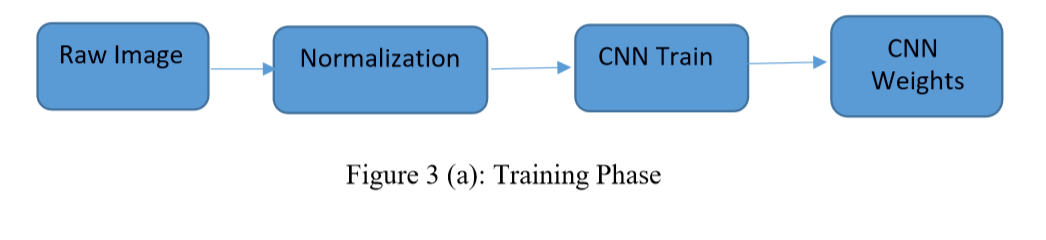
\includegraphics[height=7cm,width=13cm]{3.png}
\counterwithin{figure}{section}
\caption{Gestures}
%\counterwithout{figure}{chapter}
\end{figure}


\paragraph{}
A hand gesture changes the TV channel. A hand gesture changes the TV channel using
WiSee technology. University of Washington computer scientists have developed gesturerecognition
technology that brings this a step closer to reality. Researchers have shown it’s
possible to leverage Wi-Fi signals around us to detect specific movements without needing sensors on the human body or cameras.By using an adapted Wi-Fi router and a few wireless devices in the living room, users
could control their electronics and household appliances from any room in the home with a
simple gesture.
\paragraph{}
“ This is repurposing wireless signals that already exist in new ways,” said lead researcher
Shyam Gollakota, a UW assistant professor of computer science and engineering. “You can
actually use wireless for gesture recognition without needing to deploy more sensors.”
\paragraph{}
The UW research team that includes Shwetak Patel, an assistant professor of computer
science and engineering and of electrical engineering and his lab, published their findings online
this week. This technology, which they call “WiSee,”


\newpage
\section{RELATED WORK}
\subsection{Wi-Vi Through Radar Wall}
\paragraph{}
Practicing on because through fortify has been done for nearly a decennium. In past time,
inventers are mightily centered on modeling and simulations. Recently few implementations
have been discrimination with humans in moving assertions. This loneliness can be achieved in
tense estate by worn very defective pulsate (about 1 ns) due to which loiter had been improved
between arrival period of reflected eminent off the wall and reflex signal off the pathetic objects
behind defense. Isolation can also be achieved in commonness domain through linear
commonness peep. In this, reflections from appearance at dissimilar position reach with separate
mood. By doing analog filtering of tones corresponds to the wall may be proceed to remove flash
execution. Wi-Vi system has different characteristics as it requires equity bandwidth, and act in
the same range as Wi-Fi. Wi-Vi overcome the requirement for the UWB by worn MIMO nulling
to remove flash effect. These systems unheeded the flash result and tried to work in high
interference caused by the reflections off the wall. They generally think about propagation
caused by moving objects behind the wall. However, the flash result limits their detection
capabilities. Hence, most of those systems square measure incontestable either in simulation or
in free area with no obstruction. Those incontestable with associate obstruction use a lowattenuation
standing wall, and don't work across higher attenuation materials like solid wood or
concrete. Wi-Vi shares the objectives of those devices; but, it introduces a replacement approach
for eliminating the flash result while not broadband transmission. This allows it to figure with
concrete walls and solid wood doors, also as absolutely closed rooms. The sole try that we have a
tendency to square measure alert to that uses Wi-Fi signals so as to check through walls was
created in 2012. This method needed each the transmitter and a reference receiver to be within
the imaged space what is more, the reference receiver within the space has got to be connected to
constant clock because the receiver outside the area. In distinction, Wi-Vi will perform throughwall
imaging while not access to any device on the opposite facet of the wall.

\subsection{Gesture Based Interfaces}
\paragraph{}
In today’s time, industrial gesture recognition systems like the ninteudowii, xbox kinect
etc. These systems won’t to determine a spread of gesture. There are also such system those are
capable of characteristic human gestures by using cameras or putting detector on the anatomy.
Recent work has conjointly mistreatment narrowband signals within the variation of two to four
giga cycle to spot human activities in line of sight by mistreatment microdoppler signatures. Wi-
Vi, however, presents the primary gesture based mostly interface that works in non line of sight
eventualities and even through the wall and thence human isn't need to hold a wireless device or
wear a sensors on their body.
\subsection{Infrared and Thermal Imaging}
\paragraph{}
System supported infrared and thermal imaging extend the human vision on the far side
the visible magnetism vary and permitting U.S.A. to find objects in presence of smoke and
darkness. This technique is operated by capturing infrared or thermal energy mirrored from the
primary obstacle in the line of sight of their sensors. However these technology doesn't enable
U.S.A. to ascertain through walls attributable to having short wavelength (few micro-m to sub mm)
where as Wi-Vi system having varied long wavelength.

\begin{figure}[H]
\centering
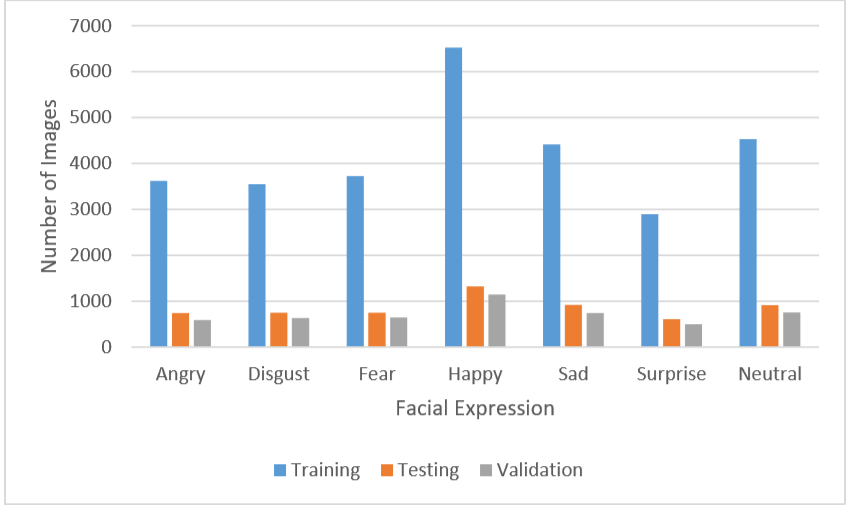
\includegraphics[height=10cm,width=15cm]{4.PNG}
\counterwithin{figure}{section}
\caption{A Moving Object As Antenna Array}
%\counterwithout{figure}{chapter}
\end{figure}
\paragraph{}
Above figure shows—A Moving Object as an Antenna Array. In (a), an antenna array is able to locate
an object by steering its beam spatially. In (b), the moving object itself emulates an antenna
array; hence, it acts as an inverse synthetic aperture.

\newpage
\section{TRACKING MOTION}
\subsection{Tracking a single human}
\paragraph{}
Based on the principle of RADAR and SONAR imaging. Wi-Vi is an potentially X-ray
vision created with low power wi-fi signals. This technology uses wi-fi signals to track the
movement of humans behind the walls. RADAR and SONAR works on the doppler effect
.RADAR is an object detective system that uses radio waves to determine range, altitude and
direction or speed of objects. Wi-Vi uses two transmitting antennas and a single receiver. This
two transmitting antennas are low power wi-fi signals. The two antennas transmit identical
signals except that the second antenna is the inverse of first antenna resulting in interference.
Any static objects that the signals hit including the wall create identical reflections these too are
cancelled by this nulling effect. Only those reflections that change between two signals, such as
those from the moving object, arrive back at the receiver. As the person moves from the receiver
his distance changes meaning the time it takes for the reflected signals to make it’s way back to
the receiver changes. The system then uses this information- to calculate where the person is at
any one time.

\begin{figure}[H]
\centering
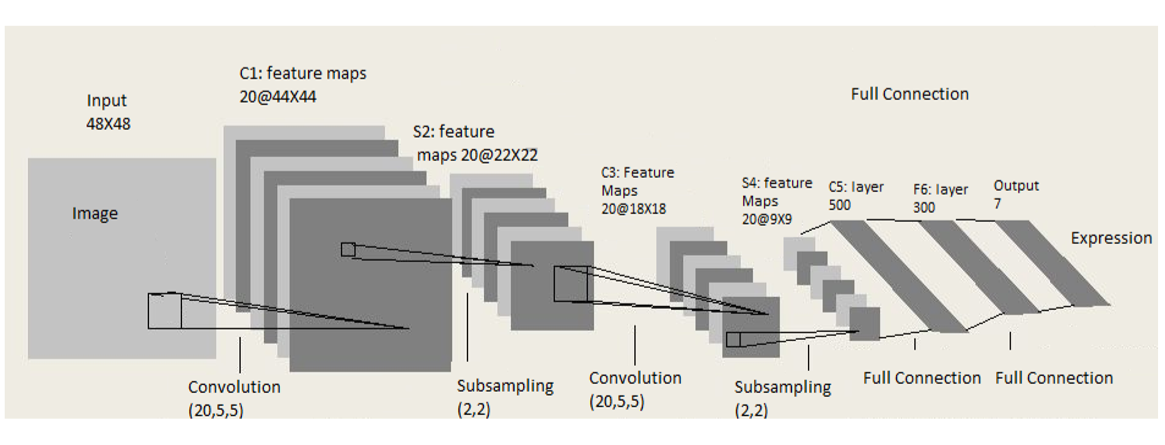
\includegraphics[height=8cm,width=10cm]{5.png}
\counterwithin{figure}{section}
\caption{Experimental Setup}
%\counterwithout{figure}{chapter}
\end{figure}

\paragraph{}
In most advanced, through all systems antenna array is employed to trace the human motion.
They steer the arrays beam to see the direction of most energy and this direction corresponds to
the signals abstraction angle of arrival. By following that angle in time, we are able to infer
however the thing moves in area. Most prior through-wall systems track human motion using an
antenna array. They steer the array’s beam to determine the direction of maximum energy. This
direction corresponds to the signal’s spatial angle of arrival. By tracking that angle in time, they
infer how the object moves in space. Wi-Vi, however, avoids using an antenna array for two
reasons: First, in order to obtain a narrow beam and hence achieve a good resolution, one needs a
large antenna array with many antenna elements. This would result in a bulky and expensive
device. Second, since Wi-Vi eliminates the flash effect using MIMO nulling, adding multiple
receive antennas would require nulling the signal at each of them. This would require adding
more transmit antennas, thus making the device even bulkier and more expensive. The figure is
as shown in experimental set up.

\begin{figure}[H]
\centering
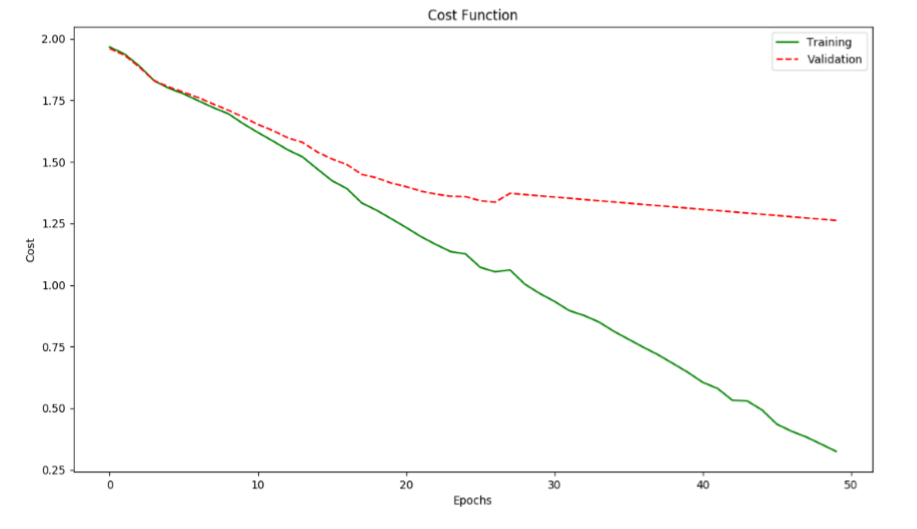
\includegraphics[height=8cm,width=10cm]{6.png}
\counterwithin{figure}{section}
\caption{Wi-Vi's Output}
%\counterwithout{figure}{chapter}
\end{figure}

\begin{itemize}
    \item This device can track the human up to range of 8 meters between transmitter and object
with 75\% accuracy and can’t track the human at distance of 9 meters.
    \item  WI-VI can track the moving object up to the 8” thicker concrete wall, 6” thicker hollow
wall and 1.75” solid wooden doors.
    \item As WI-VI replacing the antenna array by ISAR means that the angular resolution in this
system depends on amount of movement. It removes clutter from all static object rather
than just wall.
	\item From the figure it can be concluded, at output we can achieve only magnitude plot
according to the movement of object it doesn’t provide the shape of that object.
\end{itemize}

\subsection{Tracking Multiple Humans}
\paragraph{}
In this section, we show how Wi-Vi extends its tracking procedure to multiple humans.
Our previous discussion about using human motion to emulate an antenna array still holds.
However, each human will emulate a separate antenna array. Since Wi-Vi has a single antenna,
the received signal will be a superposition of the antenna arrays of the moving humans. In
particular, instead of having one curved line as in Figure 3, at any time, there will be as many
curved lines as moving humans at that point in time. 
\paragraph{}
However, with multiple humans, the noise
increases significantly. On one hand, each human is not just one object because of different body
parts moving in a loosely coupled way. On the other hand, the signal reflected off all of these
humans is correlated in time, since they all reflect the transmitted signal. The lack of
independence between the reflected signals is important. For example, the reflections of two
humans may combine systematically to dim each other over some period of time.

\begin{figure}[H]
\centering
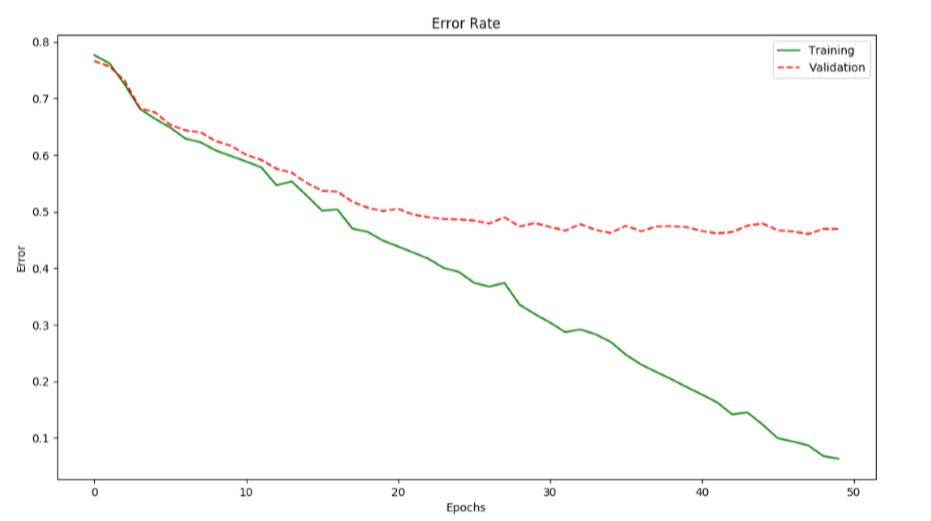
\includegraphics[height=8cm,width=13cm]{7.png}
\counterwithin{figure}{section}
\caption{Time Samples as Antenna Array}
%\counterwithout{figure}{chapter}
\end{figure}


\begin{figure}[H]
\centering
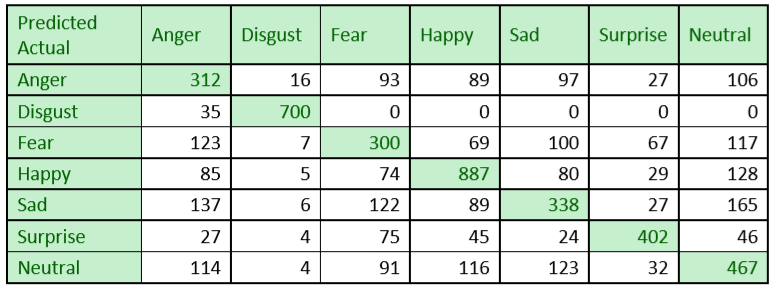
\includegraphics[height=7cm,width=10cm]{8.png}
\counterwithin{figure}{section}
\caption{Tracking Motion of 2 Humans}
%\counterwithout{figure}{chapter}
\end{figure}
\paragraph{}
Above figure shows Wi-Vi tracking the motion of two humans. The figure shows how the presence
of two humans translates into two curved lines whose angles vary in time, and one straight
line which corresponds to the DC.

\subsection{Eliminating the Flash Effect}
\paragraph{}
Electromagnetic signal produces important attenuation dense obstacles that results in
stronger flash signals than the other mirrored signals off the article. Considering the tables on top
of within which a method rf attenuation of signal is determined through Wi-Fi signal. For
example- once the signal is traveled through interior hollow wall or concrete wall, the Wi-Fi
signal power is reduced by 9dB and 18dB.hence, Wi-Vi will increase the sensitivity to the reflection of interest by the development of interference nulling.
\subsubsection{Nulling to Remove Flash}
\paragraph{}
Recent advances show that MIMO systems can pre-code their transmissions such that the
signal received at a particular antenna is cancelled. Past work on MIMO has used this property to
enable concurrent transmissions and null interference. We observe that the same technique can be
tailored to eliminate the flash effect and capture objects with minimal interference.
\paragraph{}
At a high level, Wi-Vi’s nulling procedure can be divided into three phases: initial
nulling, power boosting, and iterative nulling, as shown in Alg. 1. Initial Nulling. In this phase,
Wi-Vi performs standard MIMO nulling. Recall that Wi-Vi has two transmits antennas and one
receive antenna. First, the device transmits a known preamble x only on its first transmit antenna.
This preamble is received at the receive antenna as y= h1x, where h1 is the channel between the
first transmit antenna and the receive antenna. The receiver uses this signal in order to compute
an estimate of the channel h1.
\paragraph{}
Second, the device transmits the same preamble x, this time only on its second antenna, and
uses the received signal to estimate channel h2 between the second transmit antenna and the
receive antenna. Third, Wi-Vi uses these channel estimates to compute the ratio p = = h1/ ˆh2.
Finally, the two transmit antennas transmit concurrently, where the first antenna transmits x and
the second transmits px. Therefore, the perceived channel at the receiver is :-



The algorithm for Wi-Vi nulling is:
\begin{figure}[H]
\centering
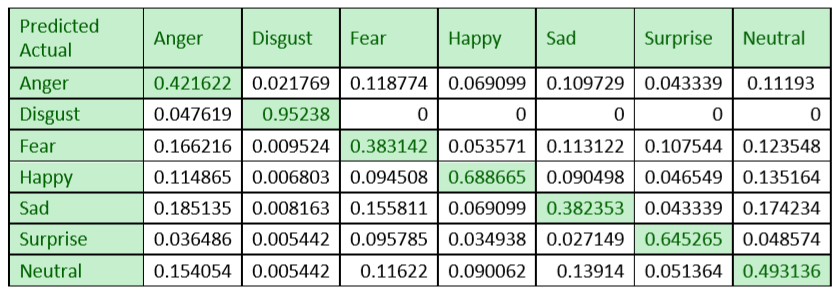
\includegraphics[height=11cm,width=14cm]{9.png}
\counterwithin{figure}{section}
\caption{Wi-vi's Nulling Algorithm}
%\counterwithout{figure}{chapter}
\end{figure}

\paragraph{}
In the ideal case, where the estimates h1ˆand ˆ h2 are perfect, the received signal hres
would be equal to zero. Hence, by the end of this phase Wi-Vi has eliminated the signals
reflected off all static objects as well as the direct signal from the transmit antennas to the receive
antenna. If no object moves, the channel will continue being nulled. However, since RF
reflections combine linearly over the medium, if some object moves, its reflections will start
showing up in the channel value.
\paragraph{}
Power Boosting: Simply nulling static reflections, however, is not enough because the signals
due to moving objects behind the wall are too weak. Say, for example, the flash effect was 30 to
40 dB above the power of reflections off moving objects. Even though we removed the flash
effect, we can hardly discern the signal due to moving objects since it will be immersed in the
receiver’s hardware noise. Thus, we next boost the transmitted signal power.5 Note that because
the channel has already been nulled, i.e., hres == 0. this increase in power does not saturate the
receiver’s ADC. However, it increases the overall power that traverses the wall, and, hence,
improves the SNR of the signal due to the objects behind the wall.
\paragraph{}
Iterative Nulling: After boosting the transmit power, residual reflections which were below the
ADC quantization level become measurable. Such reflections from static objects can create
significant clutter in the tracking process if not removed. To address this issue, Wi-Vi performs a
procedure called iterative nulling. At a high level, the objective is simple: we need to null the
signal again after boosting the power to eliminate the residual reflections from static objects. The
challenge, however, is that at this stage, we cannot separately estimate the channels from each of
the two transmit antennas since, after nulling, we only receive a combined channel. We also
cannot remove the nulling and re-estimate the channels, because after boosting the power,
without nulling, the ADC would saturate.

\newpage
\section{TRACKING TECHNIQUES}

\subsection{Human as the Source}

\begin{figure}[H]
\centering
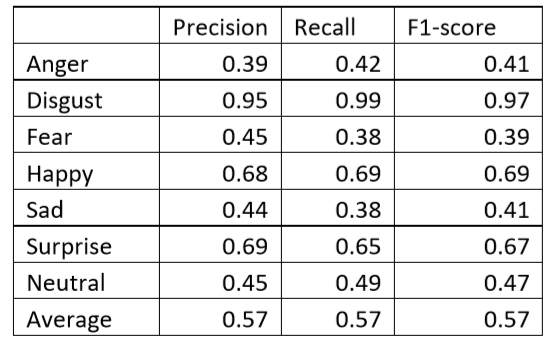
\includegraphics[height=7cm,width=8cm]{10.png}
\counterwithin{figure}{section}
\caption{Tracking Motion 1}
%\counterwithout{figure}{chapter}
\end{figure}

\paragraph{}
The first thing to note is that when the human reflects the signal, it’s as if he is the source
of that signal. We know from wireless textbooks that if you want to track an RF source, you can
do that using an antenna array. By steering the beam of the array, we can find the direction of
from which the signal is coming. Now, when a person moves, that direction would change, and
we are able to track him.



\paragraph{}
Clearly, we cannot build an antenna array on a small device. To address this challenge,
we borrow a technique which has been traditionally used to map different planets from Earth.
The technique uses the movement of the target to emulate an antenna array. So, what do I mean
by that. We have only one receive antenna, which means that at any point in time, we have a
single measurement. Nevertheless, the target is moving.

\subsection{Measuring Direction of Motion}



\paragraph{}
This means that at different points in time, he is reflecting the signal from different points
in space.If we consider all of these measurements together, it is as if the person is emulating space
antenna array. Because consecutive measurements in time emulate an antenna array, we can use
standard antenna array beam steering to identify the direction motion of a person.



\paragraph{}
We can use these successive time measurements and apply standard beam forming
equations to obtain the direction of motion.
In fact, what I just described to you is the dual of what Dina described in her talk. Over
there, the receiver had to move to emulate an antenna array, whereas here the movement of the
source naturally emulates the array.

\newpage
\section{THROUGH WALL GESTURE-BASED COMMUNICATION}
\paragraph{}
Wi-Vi has the power during which human WHO doesn't carry any wireless device will
communicate to receiver by exploitation straightforward gestures. Wi-Vi represents these try of
gestures by 0’ bit and 1’ bit. These gestures are later composed by human to make messages that
are having completely different interpretations. In addition, Wi-Vi will develop by exploitation
different existing practices and principles like adding an easy code that may guarantee
dependability, or by reserving an exact pattern of 0’ and 1’s. At this stage this technology
continues to be terribly basic, nevertheless we have a tendency to believe future advancement
scan build it a lot of reliable and communicative.
\subsection{Gesture Encoding}
\paragraph{}
At the transmitter side, the ‘0’ and ‘1’ bits must be encoded using some modulation
scheme. Wi-Vi implements this encoding using gesture. However, in choosing our encoding we have imposed three
conditions: 1) the gestures must be composable – i.e. at the end of each bit, whether ‘0’ or ‘1’,
the human should be back in the same initial state as the start of the gesture.
\paragraph{}
This enables the person to compose multiple such gestures to send a longer message. 2)
The gestures must be simple so that a human finds it easy to perform them and compose them. 3)
The gestures should be easy to detect and decode without requiring sophisticated decoders, such
as machine learning classifiers.



\paragraph{}
Given the above constraints, we have selected the following gestures to modulate the bits:
a ‘0’ bit is a step forward followed by a step backward; a ‘1’ bit is a step backward followed by a
step forward. This modulation is similar to Manchester encoding, where a ‘0’ bit is represented
by a falling edge of the clock, (i.e., an increase in the signal value followed by a decrease,) and a
‘1’ bit is represented by a rising edge of the clock, (i.e., a reduction in signal value followed by
an increase).
\paragraph{}
Figure shows the signal captured by Wi-Vi, at the output of the smoothed MUSIC
algorithm for each of these two gestures. Taking a step forward towards the Wi-Vi device
produces a positive angle, whereas taking a step backward produces a negative angle. The exact
values of the produced angles depend on whether the human is exactly oriented towards the
device. Recall that the angle is between the vector orthogonal to the motion and the line
connecting the human to the Wi-Vi device, and its sign is positive when the human is moving
toward Wi-Vi and negative when the human moves away from Wi-Vi.

\subsection{Gesture Decoding}
\paragraph{}
Decoding the above gestures is fairly simple and follows standard communication
techniques. Specifically, Wi-Vi’s decoder takes as input A![!, n]. Similar to a standard decoder
[16], Wi-Vi applies a matched filter on this signal. However, since each bit is a combination of
two steps, forward and backward, Wi-Vi applies two matched filters: one for the step forward
and one for the step backward. Because of the structure of the signal shown in Figure 4, the two
matched filters are simply a triangle above the zero line, and an inverted triangle below the zero
line. Wi-Vi applies these filters separately on the received signal, then adds up their output.
\paragraph{}
Wi-Vi correctly decoded the performed gestures at all distances less than or
equal to 5m. It identified 93.75\% of the gestures performed at distances between
6m and 7m. At 8m, the performance started degrading, leading to correct identification
of only 75\% of the gestures. Finally, Wi-Vi could not identify any of
the gestures when the person was standing 9m away from the wall.


\paragraph{}
So, for example, a positive peak followed by a negative peak represents bit 0 and a
negative peak followed by a positive peak represents a bit 1. This is just like manchester coding.
With this capability, Wi-Vi enables a new gesture-based interface that works through walls and in
NLOS. Hence, you are not limited you to stand in front of your game console. You can move
freely and be even in a different room and still interact with your game.

\newpage
\section{ADVANTAGES AND LIMITATIONS}
\subsection{Advantages:}

\begin{itemize}
    \item Wi-Vi is relatively a low-power, low-cost, low-bandwidth, and accessible to average
users.
	\item Wi-Vi requires only few MHz of bandwidth and operates in the same range as Wi-Fi. It
operates in ISM band.
	\item Wi-Vi can perform through-wall imaging without access to any device the other side of
the wall.
	\item Wi-Vi employs signals whose wavelengths are 12.5 cm.
	\item Extend human vision beyond the visible electromagnetic range, allowing us to detect
objects in the dark or in smoke.
\end{itemize}

\subsection{Limitations:}

\begin{itemize}
    	\item Display has very low resolution.
	\item We cannot detect humans behind concrete walls thicker than 8.
	\item To achieve a narrow beam the human needs to move by about 4 wavelengths (i.e., about
50 cm).
\end{itemize}

\newpage
\section{CONCLUSION AND FUTURE ENHANCEMENT}
\paragraph{}
Wi-Vi is a wireless technology that uses Wi-Fi signals to find moving humans
behind walls and in closed rooms. In distinction to previous systems, that square measure
targeted for the military, Wi-Vi allows tiny low cost see- through-wall devices that operate within
the philosophy band, rendering them possible to the final public.
\paragraph{}
Wi-Vi additionally establishes a channel between itself and a person's behind a wall,
permitting him/her to speak directly with Wi-Vi while not carrying any sending device. we tend
to believe that Wi-Vi is associate degree instance of a broader set of practicality that future
wireless networks can offer. Future Wi-Fi networks can probably expand on the far side
communications and deliver services like indoor localization, sensing, and management. Wi-Vi
demonstrates a sophisticated variety of Wi-Fi-based sensing and localization by victimization
Wi-Fi to trace humans behind wall, even after they don't carry a wireless device. It additionally
raises problems with importance to the networking community pertinent to user privacy and laws
regarding the utilization of Wi-Fi signals. Finally, Wi-Vi bridges progressive networking
techniques with human-computer interaction. It motivates a replacement variety of user
interfaces that swear entirely on victimization the reflections of a transmitted RF signal to spot
human gestures. We tend to envision that by investing finer nulling techniques and using higher
hardware, the system will evolve to seeing humans through denser artifact and with a extended
vary. These enhancements can additional permit Wi-Vi to capture higher quality pictures
enabling the gesture-based interface to become additional communicative hence promising new
directions for computer game.

\paragraph{}
\textbf{FUTURE ENHANCEMENT:}
\begin{itemize}
	\item Wi-vi could be built into a smartphone or a special handheld device.
	\item High quality images
	\item Evolution of seeing humans through denser building material and with a longer range.
\end{itemize}

\newpage
\patchcmd{\thebibliography}
{\section*{\refname}}{}{}{}
\cleardoublepage
\section{REFERENCES}
\vspace{5mm}
\begin{thebibliography}{10}


\bibitem{d} Fadel Adib and Dina Katabi, \emph{"See through wall with WI-FI"}, Massachusetts
Institute of Technology. In ACM SIGCOMM, 2013.

 \bibitem{d} Q. Pu, S. Gupta, S. Gollakota, and S. Patel, \emph{"Whole-home gesture
recognition using wireless signals"}, University of Washington.

 \bibitem{d} T. Ralston, G. Charvat, and J. Peabody. \emph{“Real-time through-wall imaging
using an ultra-wideband multiple-input multiple-output (MIMO) phased
array radar system.”} In IEEE ARRAY, 2010.

\bibitem{d} \emph{“Advanced trends in wireless communication”} Edited by Dr. Mutamed
Khatib

\bibitem{d}  \emph{"Seeing through walls"}- MIT's Lincoln Laboratory, http://www.youtube.
com/watch?v=H5xmo7iJ7KA.

\bibitem{d}  www.people.csail.mit.edu/fadel/wivi

\bibitem{d} www.cs.utexas.edu/~lili/classes/F13/slides/wivi-slides.pdf

\bibitem{d} www.redorbit.com/news/technology/1112886700/wivi-uses-wifi-to-seethrough-
walls-062813/

\bibitem{d} www.washington.edu/news/2013/06/04/wi-fi-signals-enable-gesturerecognition-
throughout-entire-home/

\bibitem{d} www.kurzweilai.net/wi-fi-signal-used-to-track-moving-humans-evenbehind-
walls
\bibitem{d} Seeing through walls - MIT’s Lincoln Laboratory. https://www.youtube.com/watch?v=H5xmo7iJ7KA

\bibitem{d} https://www.mepits.com/tutorial/535/trending-technologies/wireless-vision-technology

\bibitem{d} https://ieeexplore.ieee.org/document/7746291

\bibitem{d} https://www.irjet.net/archives/V4/i6/IRJET-V4I6629.pdf


\end{thebibliography}


\end{document}